\chapter{Marco Teórico y Referencial}\label{chapter:marco-teorico-referencial}


El presente capítulo establece los fundamentos conceptuales y tecnológicos que sustentan el desarrollo del sistema. El estado del arte revisa las plataformas de farmacovigilancia digital existentes e identifica sus brechas. Los fundamentos de sistemas web y de bases de datos definen la arquitectura y los principios que garantizan la integridad de la información clínica. El capítulo concluye con un análisis comparativo de las tecnologías disponibles para la implementación, cuyos resultados orientan la selección del conjunto de herramientas del sistema.


\section{Marco Referencial (Estado del Arte)}

El marco referencial de este trabajo examina soluciones existentes para la notificación de eventos adversos, desde plataformas genéricas hasta sistemas nacionales de farmacovigilancia, con el fin de identificar sus limitaciones y extraer buenas prácticas que orienten el diseño del sistema ESAVI del IFV.

\subsection{Limitaciones de plataformas genéricas (Google Forms)}

El uso de plataformas de formularios en la nube como Google Forms, Microsoft Forms o JotForm podría considerarse una alternativa rápida para la captura de eventos adversos. Sin embargo, sus características las inhabilitan como solución para un sistema nacional de farmacovigilancia:

\begin{itemize}

\item \textbf{Soberanía de los datos:} La información de salud reside en servidores externos bajo jurisdicciones extranjeras, vulnerando el principio de residencia de datos clínicos que exige el marco regulatorio nacional.

\item \textbf{Validación clínica insuficiente:} Solo ofrecen validaciones básicas (campos obligatorios, formatos). Carecen de capacidad para integrar codificación clínica estandarizada o para implementar reglas de negocio complejas como la coherencia cronológica entre vacunación y aparición de síntomas.

\item \textbf{Ausencia de control de acceso granular:} No permiten definir roles diferenciados (reportante, médico evaluador, jefe de vacunación) con permisos específicos, lo cual es indispensable en un flujo de farmacovigilancia.

\item \textbf{Falta de trazabilidad:} No registran quién modificó un reporte ni cuándo, imposibilitando la auditoría de los datos.

\item \textbf{Interoperabilidad nula:} Los datos requieren exportación manual a hojas de cálculo, impidiendo la integración automatizada con sistemas de información de salud.

\end{itemize}

En consecuencia, estas plataformas son adecuadas para encuestas, pero no para un sistema de autorreporte de ESAVI que requiere seguridad, estructuración, trazabilidad e interoperabilidad. Esta brecha justifica el desarrollo de una solución específica.

\subsection{Análisis de sistemas de autorreporte de eventos adversos existentes}

Los sistemas de autorreporte de eventos adversos operan bajo dos modelos. 
La vigilancia pasiva depende de la iniciativa voluntaria del ciudadano o profesional para notificar un evento. 
La vigilancia activa, en cambio, contacta proactivamente al usuario mediante encuestas digitales para recopilar datos en tiempo casi real.

Este apartado examina cuatro sistemas —VAERS, NotificaRAM, V-safe y el formulario del CECMED— con el objetivo de identificar brechas de diseño que fundamenten la propuesta del sistema ESAVI-IFV.

\subsubsection{Sistema de Notificación de Eventos Adversos a Vacunas (VAERS, por sus siglas en inglés)}

\textbf{VAERS} es el sistema nacional de farmacovigilancia en los Estados Unidos, administrado por la Administración de Alimentos y Medicamentos (FDA, por sus siglas en inglés), agencia reguladora de medicamentos y alimentos, y los Centros para el Control y la Prevención de Enfermedades (CDC, por sus siglas en inglés), organismo responsable del control y prevención de enfermedades \cite{fda_vaers}.
Su objetivo principal es detectar señales de seguridad no identificados durante los ensayos clínicos \cite{cdc_vaers}.

Permite la notificación voluntaria de eventos adversos por parte de profesionales de la salud, fabricantes y ciudadanos mediante formularios web y PDF descargables \cite{vaers_official}.
Para garantizar la integridad del repositorio, la legislación estadounidense contempla sanciones civiles y penales ante el suministro intencional de información falsa en los reportes \cite{vaers_official}. 
Esto contribuye a reducir la introducción de datos malintencionados en un sistema de acceso público.

Los reportes alimentan la base de datos CDC WONDER\footnote{CDC WONDER (Wide-ranging Online Data for Epidemiologic Research): plataforma de los CDC para el acceso público a datos epidemiológicos anonimizados.}, garantizando la transparencia mediante su disponibilidad abierta \cite{vaers_official}. 
Ante una señal de alerta, el monitoreo escala hacia sistemas complementarios de vigilancia activa y evaluación clínica como VSD\footnote{Vaccine Safety Datalink (VSD): red de vigilancia que integra datos de múltiples organizaciones sanitarias para el análisis de seguridad vacunal.} y el proyecto CISA\footnote{Clinical Immunization Safety Assessment (CISA): iniciativa orientada a la evaluación clínica especializada de eventos adversos asociados a la vacunación.} para confirmar posibles riesgos \cite{cdc_vaers}.

El formulario consta de 28 secciones con un nivel de detalle que puede resultar abrumador para un usuario que reporta bajo condiciones de malestar físico. 
Además, información que en el sistema de salud cubano resulta relevante para la evaluación clínica —como síntomas, su intensidad y desenlace— termina resumida en campos de texto libre, lo que genera datos heterogéneos y difíciles de analizar de forma automatizada.


\subsubsection{NotificaRAM}

\textbf{NotificaRAM} es la plataforma oficial de farmacovigilancia en España para la notificación de sospechas de reacciones adversas a medicamentos \cite{aemps_manual_2025}.
\textit{La Agencia Española de Medicamentos y Productos Sanitarios (AEMPS)} gestiona este portal en el marco del Sistema Español de Farmacovigilancia de Medicamentos de Uso Humano (SEFV-H) \cite{aemps_sefv_2025}.

El sistema funciona de forma descentralizada, remitiendo los reportes a los Centros Autonómicos de Farmacovigilancia para su validación técnica inicial \cite{aemps_manual_2025}. 
Tras esta evaluación, la base de datos \textit{FEDRA(Farmacovigilancia Española, Datos de Reacciones Adversas)}, sistema nacional de notificación y almacenamiento de sospechas de reacciones adversas a medicamentos, centraliza todos los registros del país \cite{aemps_fedra_2026}.
Estos registros alimentan la plataforma europea EudraVigilance\footnote{EudraVigilance: sistema de la Agencia Europea de Medicamentos (EMA) para la gestión de notificaciones de reacciones adversas en la Unión Europea.} y la base de datos mundial VigiBase\footnote{VigiBase: base de datos global de reportes de seguridad, gestionada por el Centro de Monitoreo de Uppsala bajo la OMS.}, que consolidan reportes de múltiples países para la detección de señales de seguridad a nivel internacional \cite{aemps_notificacion_2026}.


Para la identificación de medicamentos, NotificaRAM emplea un sistema de búsqueda por código que sugiere posibles valores y evita cargar catálogos extensos, aunque resulta poco práctico si el notificador desconoce el código. A pesar de esta validación puntual, el formulario aún conserva numerosos campos de texto libre. Al igual que otros sistemas pasivos, depende de la iniciativa voluntaria del notificador, lo que conlleva subregistro.

\subsubsection{Formulario de notificación de \gls{ram} del \gls{cecmed} (Cuba)}

El CECMED, como autoridad reguladora de Cuba, pone a disposición un formulario para la notificación voluntaria de sospechas de reacciones adversas a medicamentos (RAM), que abarca también a las vacunas como categoría de medicamento \cite{cecmed_ram}.
A través de este formulario, el CECMED recolecta información sobre eventos adversos para alimentar la base nacional de farmacovigilancia y cumplir con su función de monitoreo continuo de la seguridad de los medicamentos comercializados en el país.

El formulario exige pocos campos obligatorios, pero omite datos esenciales para la farmacovigilancia vacunal como el número de lote, la dosis o la fecha de administración. 
Sus catálogos de medicamentos y reacciones adversas resultan extensos y complejos para un usuario sin formación sanitaria. 
Tampoco solicita contacto del paciente, lo que imposibilita el seguimiento posterior. 
Con estos datos, los reportes constituyen hechos aislados que permiten sospechar sobre un medicamento, pero resultan insuficientes para establecer relaciones de causalidad.

\subsubsection{V-safe}

Los \gls{cdc} diseñaron \textbf{V-safe} como una herramienta digital para monitorear la seguridad vacunal en los Estados Unidos.
Tras su lanzamiento inicial en diciembre de 2020 para supervisar las vacunas contra la COVID-19, el sistema extendió su alcance a otras inmunizaciones, incluyendo aquellas contra el virus respiratorio sincitial (VRS) \cite{cdc_vsafe_portal}.

A diferencia de los modelos de notificación espontánea, V-safe emplea un enfoque de vigilancia activa mediante el contacto proactivo con los usuarios. 
El sistema envía encuestas digitales por mensajes de texto o correo electrónico para recopilar información directamente del paciente \cite{cdc_about_vsafe}.
El seguimiento incluye encuestas diarias durante la primera semana posterior a la vacunación y encuestas semanales durante seis semanas adicionales \cite{cdc_vsafe_portal,vsafe_monitoring_article}. 
Esta frecuencia de contacto, aunque sistemática, puede generar fatiga en el participante.

El Anexo~\ref{app:vsafe-form-ene2021} recoge capturas representativas de la interfaz de usuario, que muestran un reporte rápido, estructurado y de baja carga sobre el estado de salud diario del usuario.

V-safe integra sistemas de vigilancia pasiva: cuando un usuario reporta la necesidad de atención médica, el sistema facilita la generación de un reporte en VAERS mediante la precarga de datos \cite{cdc_about_vsafe}.
Además, la plataforma publica los datos recopilados en formato anonimizado para su consulta en portales de acceso público.

\subsection{Análisis comparativo de los sistemas estudiados}

Este análisis compara los sistemas VAERS, NotificaRAM, V-safe y el formulario del CECMED en términos de su enfoque metodológico, actores involucrados, canales de notificación y mecanismos de captura de datos. La Tabla \ref{tab:sistemas_comparacion} sintetiza estos criterios con el objetivo de evidenciar diferencias estructurales en los modelos actuales de farmacovigilancia.

\begin{table}[htbp]
\centering
\caption{Comparación de sistemas de autorreporte de eventos adversos}
\label{tab:sistemas_comparacion}
\renewcommand{\arraystretch}{1.3}
\begin{tabular}{p{2.8cm} p{2.7cm} p{2.7cm} p{2.7cm} p{2.7cm}}

\textbf{Criterio} & \textbf{VAERS} & \textbf{NotificaRAM} & \textbf{V-safe} & \textbf{CECMED}\\[6pt]

		Tipo de vigilancia &
		Pasiva  &
		Pasiva  &
		Activa  &
		Pasiva \\[6pt]
		\hline

		Actores &
		Profesionales de salud, fabricantes y ciudadanos &
		Profesionales de salud y ciudadanos &
		Usuarios vacunados registrados &
		Profesionales, ciudadanos, industria y distribuidor\\[6pt]
        \hline
		
		Canal de notificación &
		Formularios web y PDF descargable &
		Formulario web &
		Encuestas digitales (SMS y correo electrónico) &
		Formulario web\\[6pt]
        \hline
		
		Validación clínica inicial &
No &
Sí (centros autonómicos) &
No &
No \\[6pt]
\hline
		
		Estructuración del dato &
		Texto libre; baja estandarización &
		Campos definidos; control parcial; búsqueda por código &
		Formularios digitales con validación y opciones predefinidas &
		Campos estructurados; catálogos extensos
		\\[6pt]
        \hline


		Retroalimentación al reportante &
No &
No &
Sí (seguimiento longitudinal) &
No \\[6pt]
\hline
		
		
	Limitaciones &
Subregistro; formulario extenso (28 secciones); texto libre que dificulta el análisis automatizado &
Subregistro; dependencia del notificador; búsqueda por código poco práctica sin conocerlo &
Fatiga del usuario; limitada representatividad &
Sin especificidad para vacunas; ambigüedad en roles; sin seguimiento; sin validación de coherencia \


	\end{tabular}
\end{table}



Todos comparten un rasgo común: son plataformas gubernamentales administradas por las entidades reguladoras de sus respectivos países —FDA y CDC en VAERS, AEMPS en NotificaRAM, CDC en V-safe y CECMED en Cuba—. VAERS, NotificaRAM y V-safe exigen al usuario la aceptación expresa de un aviso de privacidad; el formulario del CECMED, en cambio, no incluye este mecanismo.

En conjunto, los cuatro sistemas representan soluciones consolidadas de farmacovigilancia, pero ninguno fue diseñado para el contexto del sistema de salud cubano ni para los protocolos de un fabricante específico como el Instituto Finlay de Vacunas.
Las brechas derivadas de esta falta de adecuación, así como las directrices de diseño que de ellas emanan, aparecen en la siguiente sección.



\subsection{Síntesis de brechas y directrices para el sistema de ESAVI-IFV}


El análisis de los sistemas VAERS, NotificaRAM, V-safe y el formulario del CECMED ha permitido identificar un conjunto de brechas estructurales que limitan la aplicabilidad directa de estos modelos al contexto del sistema de salud cubano y, en particular, al Programa Nacional de Inmunización.

\subsubsection{Brechas identificadas}

\begin{enumerate}

\item \textbf{Falta de validación clínica inicial:} VAERS, V-safe y el CECMED incorporan reportes sin revisión médica previa. Solo NotificaRAM realiza una validación descentralizada, pero su modelo autonómico no es directamente replicable en Cuba.

\item \textbf{Estructuración insuficiente o inadecuada de los datos:} VAERS depende del texto libre; los catálogos del CECMED y la búsqueda por código de NotificaRAM resultan complejos para un usuario sin formación sanitaria. Estas estrategias generan datos heterogéneos o difíciles de capturar.

\item \textbf{Falta de retroalimentación al reportante:} Salvo V-safe, ningún sistema informa al usuario sobre el resultado de su notificación ni le ofrece seguimiento, lo que reduce la confianza y la motivación para reportar.

\item \textbf{Falta de especialización para un fabricante:} 
Ningún sistema está diseñado para un fabricante específico. El CECMED incluye vacunas cubanas, pero dentro de un catálogo general de medicamentos, sin adaptarse a los protocolos particulares del Instituto Finlay de Vacunas.

\item \textbf{Desalineación con el flujo de trabajo del MINSAP:} 
El CECMED recoge provincia y municipio, pero no contempla las áreas de salud ni establece roles diferenciados: los reportes alimentan directamente la base nacional sin pasar por una validación clínica municipal. VAERS, NotificaRAM y V-safe carecen por completo de la estructura organizativa del sistema de salud cubano.

\end{enumerate}

\subsubsection{Directrices de diseño derivadas del análisis}

A partir de las brechas identificadas, el análisis establece las siguientes directrices para el sistema ESAVI-IFV:

\begin{enumerate}[label=\textbf{D-\arabic*}]
\item \textbf{Validación clínica descentralizada:} Incorporar un flujo donde un médico evaluador del municipio correspondiente revise cada reporte y establezca la causalidad, adaptando el modelo de NotificaRAM a la estructura del MINSAP.

\item \textbf{Captura de datos mínima pero suficiente:} Recoger los datos esenciales para la evaluación de causalidad —sujeto vacunado, vacuna, lote, dosis, evento adverso y reportante— organizados por secciones, como hacen VAERS y NotificaRAM.

\item \textbf{Catálogos reducidos y especializados:} Limitar las vacunas a las del Instituto Finlay y del esquema nacional objeto de estudio, con eventos adversos en listas predefinidas, minimizando el texto libre.

\item \textbf{Interfaz usable bajo malestar físico:} Formulario breve, con campos estructurados, que pueda completarse en pocos minutos.

\item \textbf{Retroalimentación al reportante:} Informar al usuario sobre el estado de su reporte y el resultado de la evaluación médica, tomando como referencia el seguimiento de V-safe.

\item \textbf{Consentimiento informado:} Incluir la aceptación expresa del uso de datos con fines de farmacovigilancia, como hacen VAERS, NotificaRAM y V-safe.

\item \textbf{Alineación con el MINSAP:} Reflejar los niveles de consultorio, área de salud y municipio en los roles, permisos y flujos de trabajo.
\end{enumerate}

Estas directrices constituyen la base conceptual para el diseño del sistema ESAVI-IFV, cuyo desarrollo metodológico, arquitectónico y de base de datos aparece detallado en el Capítulo \ref{chapter:proposal}.


\section{Fundamentos de sistemas web}

Una vez identificadas las brechas de los sistemas de farmacovigilancia actuales y establecidas las directrices de diseño, corresponde definir las bases conceptuales que sustentarán la solución.

El sistema propuesto pertenece al dominio de las aplicaciones web, un paradigma donde la lógica de negocio y la interfaz de usuario residen en componentes diferenciados que colaboran a través de una red. 
Antes de analizar las tecnologías concretas disponibles para cada uno de estos componentes, es necesario establecer los fundamentos que describen su arquitectura, sus roles y sus mecanismos de comunicación.

\subsection{Arquitectura cliente-servidor.}

Las aplicaciones web modernas siguen el modelo cliente-servidor. 
En este modelo, el sistema consta de dos componentes que residen en máquinas distintas y mantienen comunicación a través de una red. 
El cliente —típicamente un navegador web— solicita recursos o servicios y presenta la información al usuario mediante una interfaz gráfica. 
El servidor —una aplicación que funciona en una máquina remota— recibe esas solicitudes, procesa la lógica de negocio, consulta o modifica los datos y devuelve una respuesta. 

\subsection{Interfaz de usuario y servidor.}

En el lado del cliente opera la interfaz de usuario —denominada frontend en la literatura técnica—. 
Constituye la capa del sistema con la que el usuario interactúa directamente: presenta la información, captura datos mediante formularios y guía la experiencia de navegación. 
Funciona íntegramente en el navegador y no tiene acceso directo a la base de datos ni a la lógica de negocio. 
En el lado del servidor opera la capa de servicios —conocida como backend—, que procesa las solicitudes del usuario, ejecuta la lógica de negocio y gestiona la persistencia de los datos. 
Reside en un servidor remoto y expone sus servicios a través de una API (Application Programming Interface), un conjunto de reglas que define cómo otros programas pueden interactuar con él.

\subsection{Comunicación mediante HTTP y REST.}

La comunicación entre la interfaz de usuario y la capa de servicios ocurre mediante el protocolo HTTP (Hypertext Transfer Protocol), que establece un formato estandarizado para las solicitudes y respuestas. 
Cada solicitud del cliente incluye un método HTTP que indica la operación deseada —GET para consultar, POST para crear, PUT para modificar, DELETE para eliminar— y una URL que identifica el recurso sobre el cual opera. 
El servidor procesa la solicitud y devuelve un código de estado —200 para éxito, 201 para creación, 400 para error del cliente, 500 para error del servidor— junto con los datos solicitados.

El estilo arquitectónico REST (Representational State Transfer) refina este modelo estableciendo que cada solicitud debe contener toda la información necesaria para procesarla, sin que el servidor necesite mantener el estado de la sesión entre peticiones. 
Los datos viajan típicamente en formato JSON (JavaScript Object Notation), un formato ligero de texto que resulta legible tanto para humanos como para máquinas y que todos los lenguajes de programación modernos pueden interpretar.

\subsection{Conceptos técnicos para el análisis de tecnologías}

Para comparar las tecnologías de desarrollo, es necesario definir previamente algunos conceptos.

\begin{itemize}
	\item Marco de trabajo (framework): conjunto de bibliotecas, herramientas y convenciones que proporcionan una estructura base para el desarrollo de aplicaciones.
	\item Multiplataforma: capacidad de un entorno de desarrollo para ejecutarse en distintos sistemas operativos sin requerir modificaciones en el código fuente.
	\item Entorno de ejecución (runtime): componente que ejecuta el código compilado y gestiona recursos como la memoria y los hilos de ejecución.
	\item Middleware: componente de software que procesa una solicitud HTTP encadenándose con otros componentes para validarla, autenticarla o transformarla antes de que alcance la lógica de negocio.
	\item Inyección de dependencias (DI): patrón de diseño mediante el cual un objeto recibe sus dependencias desde el exterior en lugar de crearlas internamente.
\end{itemize}

\section{Fundamentos de bases de datos}

El sistema ESAVI del IFV requiere almacenar datos clínicos de forma segura, consistente y trazable. 
Para fundamentar las decisiones de diseño de la capa de datos, a continuación aparecen los conceptos esenciales que sustentan el modelo de base de datos seleccionado.

\subsection{Modelo relacional}

El modelo relacional organiza los datos en tablas (relaciones) compuestas por filas (tuplas) y columnas (atributos). Cada tabla representa una entidad del dominio y las relaciones quedan definidas mediante claves foráneas.
Este modelo, propuesto por Codd en 1970, constituye la base de los sistemas de gestión de bases de datos relacionales (SGBDR) y sigue siendo el estándar para aplicaciones que requieren integridad y consistencia de los datos \cite{codd1970}.

\subsection{Propiedades ACID}

Las propiedades ACID garantizan la fiabilidad de las transacciones en una base de datos relacional \cite{ibm_acid_properties}:

\begin{itemize}
	\item \textbf{Atomicidad:} Una transacción ocurre por completo o no ocurre en absoluto. Si un fallo interrumpe el proceso, el sistema no almacena datos parciales.
    \item \textbf{Consistencia:} Cada transacción lleva la base de datos de un estado válido a otro, respetando todas las reglas de integridad definidas.
    \item \textbf{Aislamiento:} Las transacciones concurrentes no interfieren entre sí. El reporte de un usuario no afecta los datos de otro reporte en curso.
    \item \textbf{Durabilidad:} Una vez confirmada una transacción, sus efectos persisten incluso ante fallos del sistema.
\end{itemize}

Estas propiedades son especialmente relevantes en un sistema de farmacovigilancia, donde la integridad de los reportes de eventos adversos tiene implicaciones para la seguridad de la población.

\subsection{Propiedades BASE y teorema CAP}

En contraste con el modelo ACID, las bases de datos NoSQL adoptan el modelo BASE \cite{moniruzzaman2013nosql}:

\begin{itemize}
    \item \textbf{Básicamente disponible (Basically Available):} el sistema garantiza disponibilidad de los datos en todo momento, aunque no necesariamente consistentes.
    \item \textbf{Estado blando (Soft-state):} el estado del sistema puede cambiar con el tiempo, incluso sin entrada de datos.
    \item \textbf{Consistencia eventual (Eventual consistency):} los datos alcanzarán un estado consistente en algún momento posterior, tras la propagación de las actualizaciones.
\end{itemize}

Esta elección responde al teorema CAP, el cual establece que un sistema distribuido solo puede garantizar simultáneamente dos de tres propiedades \cite{ibm_cap_theorem}: consistencia (todos los nodos ven los mismos datos al mismo tiempo), disponibilidad (el sistema responde a cada solicitud) y tolerancia a particiones (el sistema sigue operando con la red dividida).

\subsection{Escalabilidad}

La escalabilidad describe la capacidad de un sistema para manejar un incremento de carga sin degradar su rendimiento. Existen dos estrategias:

\begin{itemize}
    \item \textbf{Escalabilidad vertical:} aumentar los recursos hardware (RAM, CPU) del servidor existente. 
    \item \textbf{Escalabilidad horizontal:} agregar más servidores al sistema y distribuir la carga entre ellos. 
\end{itemize}

\subsection{Normalización}

La normalización es el proceso de organizar los datos para eliminar redundancias y dependencias inconsistentes \cite{codd1970}. 
Consiste en aplicar un conjunto de reglas (formas normales) que evitan anomalías durante la inserción, actualización o eliminación de registros. 
En un sistema de ESAVI, los datos del paciente y los datos de la vacuna residen en tablas separadas para evitar repetir información en cada reporte.


\section{Análisis de tecnologías para la implementación del sistema propuesto}
\label{section:analisis_tecnologias}

El desarrollo de sistemas informáticos orientados al dominio clínico requiere la selección de un conjunto de tecnologías que garanticen propiedades fundamentales como la confiabilidad, la integridad de los datos, la escalabilidad y la mantenibilidad del software. El presente análisis estudia diferentes alternativas tecnológicas utilizadas en la construcción de sistemas modernos, abarcando tanto el desarrollo de la capa de servicios como de la interfaz de usuario y los sistemas de gestión de bases de datos.

\subsection{Criterios técnicos para la selección de tecnologías}
\label{subsection:criterios}

La selección de estas tecnologías parte de criterios técnicos previamente definidos que permiten evaluar de forma objetiva las distintas opciones disponibles.

\begin{itemize}
    \item \textbf{Eficiencia y rendimiento:} capacidad de la tecnología para responder adecuadamente bajo cargas de trabajo variables, garantizando tiempos de respuesta adecuados en escenarios de uso intensivo.
    \item \textbf{Escalabilidad:} capacidad del sistema para adaptarse al crecimiento en el número de usuarios y volumen de datos, tanto a nivel vertical como horizontal.
    \item \textbf{Mantenibilidad:} facilidad para realizar modificaciones, extensiones o correcciones en el software sin afectar negativamente su funcionamiento global.
    \item \textbf{Madurez tecnológica:} nivel de estabilidad y uso comprobado de una tecnología, reflejado en su adopción en entornos reales, la calidad de su documentación y el soporte de su comunidad.
    \item \textbf{Curva de aprendizaje:} esfuerzo requerido para que un desarrollador adquiera competencia en la tecnología y pueda contribuir al proyecto.
\end{itemize}

Estos criterios sirven como base para el análisis comparativo presentado en las secciones siguientes.


\subsection{Tecnologías para el desarrollo de la capa de servicios}
\label{subsection:backend}

Definida la capa de servicios en la sección anterior, corresponde ahora analizar las tecnologías disponibles para su implementación. 
El objetivo no consiste en identificar la mejor solución en términos absolutos, sino en analizar tres marcos de trabajo —.NET, Spring Boot y NestJS— que representan paradigmas distintos dentro del ecosistema actual.
Cada uno aporta fortalezas aplicables al sistema de farmacovigilancia, y la elección final dependerá de su ajuste a los criterios definidos.

\subsubsection{.NET}

.NET es un framework multiplataforma de código abierto mantenido por Microsoft que utiliza C\# como lenguaje de programación principal.
Su entorno de ejecución traduce el código a instrucciones nativas mediante dos estrategias complementarias. 
La compilación JIT (Just-In-Time) convierte el código a medida que la aplicación lo ejecuta. 
La estrategia AOT (Ahead-Of-Time) realiza la conversión completa antes de la ejecución para reducir el tiempo de inicio y el consumo de memoria \cite{dotnet_official}.

ASP.NET Core, su módulo para APIs REST, organiza el procesamiento de cada solicitud mediante un conjunto de middlewares encadenados que procesan la petición antes de generar la respuesta. 
Este modelo evita la sobrecarga de hilos por conexión \cite{ms_aspnet_architecture}.

Incorpora de manera nativa un contenedor de inyección de dependencias que gestiona el ciclo de vida de los componentes sin necesidad de bibliotecas externas \cite{ms_di_doc}. 
Para el acceso a los datos, .NET integra Entity Framework Core. 
Esta herramienta permite escribir consultas en el mismo lenguaje de programación sin necesidad de aprender un lenguaje de consulta separado, lo que reduce la curva de aprendizaje \cite{ef_core_doc}.

\subsubsection{Spring Boot}

Spring Boot es un framework basado en Java que opera sobre la Máquina Virtual de Java (JVM), un entorno que ejecuta el código compilado sobre una capa de abstracción independiente del sistema operativo. 
Esta capa adicional simplifica el desarrollo, pero incrementa el consumo de memoria en estado de reposo y bajo carga en comparación con otros entornos de ejecución \cite{spring_official}.
Utiliza el paradigma de Inversión de Control (IoC) para gestionar los componentes de la aplicación, y Spring MVC para implementar APIs REST con una estructura organizada en controladores, servicios y repositorios \cite{spring_in_action}. 
Para la persistencia, integra Spring Data JPA, que abstrae el acceso a los datos y permite definir consultas mediante anotaciones directamente en el código, lo que reduce la complejidad del desarrollo.

El desarrollo con Spring Boot requiere instalar el entorno de desarrollo de Java, configurar un gestor de dependencias y familiarizarse con un ecosistema extenso de anotaciones, lo que incrementa la curva de aprendizaje en comparación con otros frameworks \cite{spring_in_action}.

\subsubsection{NestJS}

NestJS es un framework basado en Node.js y TypeScript. 
Funciona sobre el motor V8 de Google, que compila JavaScript a código máquina en tiempo de ejecución. 

Su modelo de concurrencia descansa en un bucle de eventos (event loop) de un solo hilo, lo que permite manejar miles de conexiones simultáneas sin crear un hilo por cada solicitud.
Este diseño resulta muy eficiente en operaciones de entrada/salida (I/O) y favorece la escalabilidad en escenarios con alta concurrencia de conexiones ligeras, aunque pierde rendimiento en tareas intensivas en CPU \cite{nestjs_official}.

La arquitectura del framework organiza la aplicación mediante módulos que agrupan controladores y servicios, e incorpora un sistema de inyección de dependencias propio. 
A diferencia de .NET y Spring Boot, no incluye una herramienta de persistencia integrada, sino que delega esta responsabilidad en bibliotecas externas como TypeORM o Prisma, lo que añade una dependencia adicional y puede incrementar la curva de aprendizaje.

\subsubsection{Comparación de las plataformas de desarrollo}

La Tabla \ref{tab:comparacion_backend} resume la comparación realizada según los criterios definidos en la Sección~\ref{subsection:criterios}.

\begin{table}[htbp]
	\centering
	\caption{Comparación de tecnologías para la capa de servicios según criterios de evaluación}
	\label{tab:comparacion_backend}
	\renewcommand{\arraystretch}{1.3}
	\begin{tabular}{p{3.2cm} p{3.5cm} p{3.5cm} p{3.5cm}}
	\textbf{Criterio} & \textbf{.NET} & \textbf{Spring Boot} & \textbf{NestJS} \\[6pt]
		Eficiencia & Alta (alta tasa de transferencia, menor tiempo de procesamiento, menor consumo de RAM) & Alta (rendimiento estable, mayor consumo de memoria JVM) & Media (eficiente en I/O, menor rendimiento en CPU intensivo) \\[6pt] \hline
		Escalabilidad & Alta (menor consumo de recursos por instancia, alto rendimiento bajo carga) & Muy alta (ecosistema maduro y ampliamente probado en arquitecturas distribuidas) & Alta (alta concurrencia en I/O mediante modelo no bloqueante) \\[6pt] \hline
		Mantenibilidad & Alta (DI nativo, arquitectura estructurada y tipada) & Alta (IoC consolidado, ecosistema estandarizado) & Media (ecosistema heterogéneo) \\[6pt] \hline
		Madurez & Muy alta (plataforma enterprise, soporte LTS) & Muy alta (amplia adopción empresarial) & Media (ecosistema en crecimiento) \\[6pt] \hline
		Curva de aprendizaje & Media-Alta (herramientas integradas) & Alta (ecosistema complejo) & Media-Baja (framework accesible) \\[6pt] \hline
	\end{tabular}
\end{table}

La valoración de este criterio encuentra respaldo en estudios que han medido el comportamiento de los frameworks bajo condiciones de carga controladas. 
Godinho et al. (2024) compararon el rendimiento de APIs REST implementadas en .NET y Spring Boot mediante una suite de pruebas controladas. 

Sus resultados muestran que, en estado de reposo, Spring Boot consume aproximadamente el doble de memoria RAM que .NET (1.40 GiB frente a 694 MiB), mientras que el uso de CPU es similar en ambos \cite{performance_study}. 
En cuanto al throughput —el número de respuestas por segundo que el servidor es capaz de procesar—, .NET supera consistentemente a Spring Boot bajo carga concurrente. 
Esta ventaja también aparece en los benchmarks independientes de TechEmpower\footnote{TechEmpower Framework Benchmarks es un proyecto de código abierto que ejecuta pruebas estandarizadas sobre cientos de frameworks web. Evalúa múltiples escenarios —consultas a base de datos, serialización JSON, texto plano, entre otros— midiendo el rendimiento relativo de cada tecnología bajo condiciones homogéneas de carga \cite{techempower_benchmarks}.}, que sitúan a .NET por delante de Spring Boot y de NestsJs en el escenario de múltiples consultas por solicitud .
La Figura \ref{fig:benchmark_rendimiento} muestra ambas métricas: .NET obtiene la mayor tasa de transferencia y el menor tiempo de procesamiento entre los tres frameworks, lo que fundamenta la valoración de este criterio.

\begin{figure}[htbp]
    \centering
    \begin{minipage}[b]{0.50\textwidth}
        \centering
        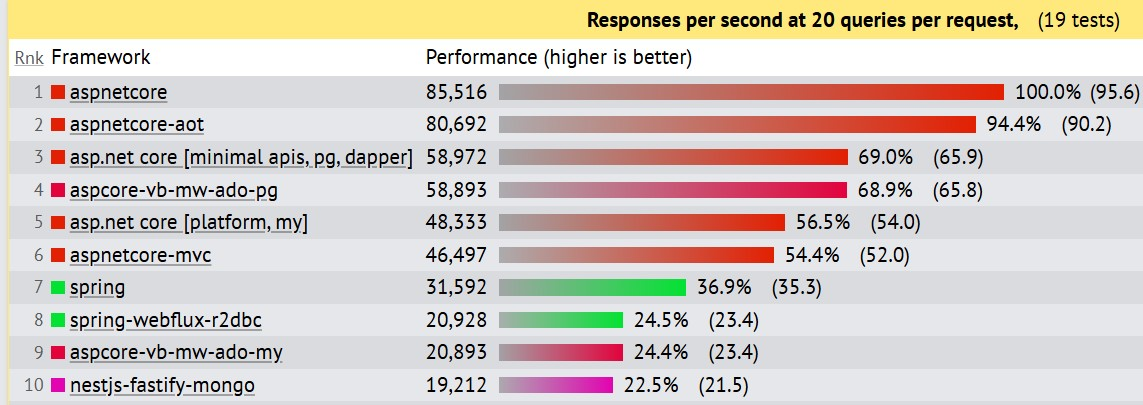
\includegraphics[width=\textwidth]{Graphics/Cap2/bencharmk_definitivo.jpg}
        \textbf{(a)} Tasa de transferencia (respuestas por segundo)
    \end{minipage}
    \hfill
    \begin{minipage}[b]{0.48\textwidth}
        \centering
        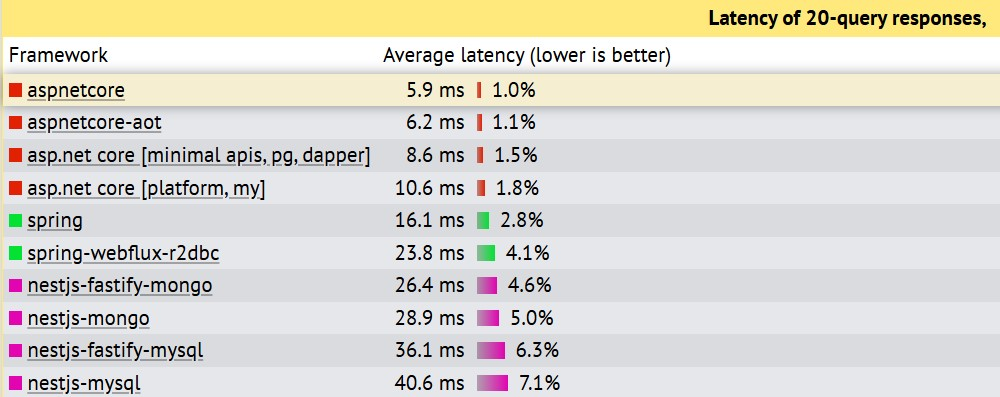
\includegraphics[width=\textwidth]{Graphics/Cap2/latencia.jpg}
        \textbf{(b)} Tiempo de procesamiento para 20 consultas
    \end{minipage}
    \caption{Comparación de rendimiento entre .NET, Spring Boot y Node.js en el escenario de 20 consultas por solicitud (adaptado de TechEmpower Framework Benchmarks \cite{techempower_benchmarks})}
    \label{fig:benchmark_rendimiento}
\end{figure}



\subsubsection{Selección de la plataforma}

A partir del análisis realizado, .NET constituye la opción más adecuada para el sistema de farmacovigilancia por las siguientes razones:

\begin{enumerate}
    \item \textbf{Eficiencia de recursos:} menor consumo de memoria y alto rendimiento bajo carga, lo que favorece su despliegue en entornos con recursos limitados \cite{performance_study}.
    \item \textbf{Fiabilidad en operación:} comportamiento estable bajo cargas sostenidas, que garantiza la integridad de las transacciones críticas \cite{performance_study}.
    \item \textbf{Ecosistema integrado:} proporciona bibliotecas nativas para seguridad, persistencia y autenticación, lo que evita la dependencia de componentes externos y facilita la evolución del sistema con soporte a largo plazo.
    \item \textbf{Adecuación al contexto:} la experiencia previa con el ecosistema .NET reduce la curva de aprendizaje y el riesgo de implementación.
\end{enumerate}

\subsection{Tecnologías para el desarrollo de la interfaz de usuario}
\label{subsection:frontend}

El análisis considera tres tecnologías representativas del desarrollo de interfaces de usuario modernas: React, Angular y Vue. La selección de estas tres responde a que representan enfoques distintos dentro del ecosistema actual —una biblioteca flexible, un framework integral y un marco progresivo—, lo que permite una comparación basada en los criterios definidos.

\subsubsection{React}

React es una biblioteca de JavaScript desarrollada por Meta para la construcción de interfaces mediante componentes reutilizables. 
Su modelo declarativo opera sobre una representación virtual del documento (Virtual DOM). En lugar de manipular directamente la estructura del navegador, React aplica los cambios sobre esta representación virtual. A continuación, un algoritmo de reconciliación calcula la diferencia mínima con el estado anterior y actualiza solo los elementos modificados.
Esta estrategia reduce las operaciones costosas de manipulación del documento y mejora el rendimiento en interfaces con alta frecuencia de cambios \cite{react_official}. 
React no impone una estructura completa; el enrutamiento y la gestión de estado recaen en bibliotecas externas, lo que otorga flexibilidad a costa de una mayor dependencia del ecosistema.

\subsubsection{Angular}

Angular es un framework de desarrollo de interfaces de usuario basado en TypeScript, mantenido por Google. 
Utiliza un mecanismo de vinculación bidireccional que sincroniza automáticamente el modelo de datos con la vista sin necesidad de manipulación manual \cite{angular_official}.
A diferencia de React, Angular constituye una solución integral que incluye enrutamiento, inyección de dependencias, manejo de formularios y herramientas de estructuración. 
Su enfoque dirigido por convenciones define una arquitectura estandarizada desde el inicio del proyecto, lo que favorece la consistencia en aplicaciones de gran escala pero incrementa la curva de aprendizaje.

\subsubsection{Vue}

Vue.js es un framework progresivo de JavaScript diseñado para la construcción de interfaces interactivas. 
Su sistema de reactividad rastrea automáticamente las dependencias entre los datos y la vista, actualizando solo los componentes afectados cuando el estado cambia \cite{vue_official}. 
Su diseño incremental permite adoptarlo de forma gradual: puede integrarse en proyectos existentes como una biblioteca ligera o utilizarse como framework completo, lo que reduce la curva de aprendizaje inicial.
Su reducido tamaño lo hace adecuado para cargas rápidas en redes con conectividad limitada.

\subsubsection{Comparación de los frameworks de interfaz de usuarios}

La Tabla \ref{tab:comparacion_frontend} resume la comparación realizada según los criterios definidos en la Sección~\ref{subsection:criterios}. 
En la interfaz de usuario, la eficiencia corresponde a la velocidad de actualización de la vista, la escalabilidad a la gestión de componentes complejos, y la mantenibilidad a la estructura del código.

\begin{table}[htbp]
	\centering
	\caption{Comparación de tecnologías para la interfaz de usuario según criterios de evaluación}
	\label{tab:comparacion_frontend}
	\renewcommand{\arraystretch}{1.3}
	\begin{tabular}{p{3.2cm} p{3.5cm} p{3.5cm} p{3.5cm}}
	\textbf{Criterio} & \textbf{React} & \textbf{Angular} & \textbf{Vue} \\[6pt]
		Eficiencia & Alta (representación virtual, actualización selectiva) & Media (detección de cambios por zonas) & Alta (reactividad basada en dependencias) \\ \hline
		Escalabilidad & Alta (componentes reutilizables) & Muy alta (arquitectura modular integrada) & Alta (composición flexible) \\ \hline
		Mantenibilidad & Alta (ecosistema flexible) & Muy alta (estructura tipada integral) & Alta (estructura progresiva) \\ \hline
		Curva de aprendizaje & Media (dependencia de bibliotecas externas) & Alta (framework integral) & Baja-Media (adopción gradual) \\ \hline
		Madurez & Muy alta (respaldada por Meta, amplia comunidad) & Muy alta (uso empresarial consolidado) & Alta (comunidad activa, ecosistema en crecimiento) \\ \hline
	\end{tabular}
\end{table}


\subsubsection{Selección del framework de interfaz de usuario}

Considerando los criterios evaluados, React presenta un equilibrio entre eficiencia, flexibilidad y mantenibilidad. Su modelo basado en componentes reutilizables y su estrategia de actualización selectiva lo hacen adecuado para interfaces con formularios dinámicos como los requeridos por el sistema de farmacovigilancia. Su ecosistema de bibliotecas externas permite cubrir los requisitos de validación, visualización de datos y diseño responsivo sin la rigidez estructural de Angular ni la menor madurez de Vue. Por estas razones, React constituye la tecnología seleccionada para el desarrollo de la interfaz de usuario.

\subsection{Sistemas de gestión de bases de datos}
\label{subsection:bases_datos}

Un sistema de gestión de bases de datos (SGBD) es un software encargado de gestionar el almacenamiento, la organización y la consulta de grandes volúmenes de información. 
Para el sistema de farmacovigilancia, el análisis aborda primero los dos paradigmas predominantes —relacional y no relacional— y posteriormente los gestores concretos dentro del paradigma seleccionado.

\begin{itemize}
\item \textbf{Bases de datos relacionales:} organizan la información en tablas con esquema rígido y utilizan el lenguaje de consulta estructurado (SQL, del inglés Structured Query Language) para acceder a los datos. Cumplen las propiedades ACID, lo que garantiza la integridad de los datos en operaciones críticas \cite{elmasri2016fundamentals}.
\item \textbf{Bases de datos no relacionales (NoSQL, del inglés Not Only SQL):} operan con esquemas flexibles y priorizan la disponibilidad y el rendimiento sobre la consistencia inmediata, siguiendo el modelo BASE \cite{moniruzzaman2013nosql}. Son adecuadas para grandes volúmenes de datos no estructurados.
\end{itemize}


\begin{table}[htbp]
	\centering
	\caption{Comparación de paradigmas de bases de datos según criterios de evaluación}
	\label{tab:comparacion_db}
	\renewcommand{\arraystretch}{1.3}
	\begin{tabular}{p{3.2cm} p{6.0cm} p{6.0cm}}
	\textbf{Criterio} & \textbf{Relacional (SQL)} & \textbf{No Relacional (NoSQL)} \\[6pt]
		Estructura de datos & Tablas con columnas y filas & Modelos basados en documentos, pares clave-valor, familias de columnas o grafos \\ \hline
		Esquema & Esquema rígido (definido antes de la inserción de datos) \cite{elmasri2016fundamentals} & Esquema flexible (puede variar entre registros) \cite{moniruzzaman2013nosql} \\ \hline
		Escalabilidad & Verticalmente escalable (aumento de recursos hardware del nodo) & Horizontalmente escalable (agregando más nodos al sistema) \\ \hline
		Integridad de los datos & Cumple con ACID (alta consistencia) \cite{ibm_acid_properties} & Cumple con BASE (mayor disponibilidad, menor consistencia) \cite{ibm_cap_theorem} \\ \hline
		Rendimiento & Alto en consultas complejas y operaciones transaccionales & Alta en grandes volúmenes de datos y operaciones de lectura/escritura rápidas \\ \hline
		Curva de aprendizaje & Media (requiere modelado relacional, normalización y dominio de SQL) & Media-Baja (menor necesidad de esquemas rígidos) \\ \hline
	\end{tabular}
\end{table}

En el sistema de farmacovigilancia, la prioridad es la integridad de la información clínica, no el manejo de grandes volúmenes de datos no estructurados. 
Las propiedades ACID de las bases de datos relacionales aseguran que cada operación concluya sin inconsistencias, lo que resulta esencial cuando los datos alimentan directamente la toma de decisiones clínicas.
Por esta razón, el paradigma relacional constituye la base del sistema. 
Las bases de datos no relacionales mantienen su vigencia para escenarios complementarios —documentos, evidencias, fotografías o mecanismos de almacenamiento en caché— donde la flexibilidad de esquema y el rendimiento en lectura predominan sobre la consistencia transaccional.

\subsubsection{Comparación de gestores de bases de datos relacionales}

Una vez seleccionado el paradigma relacional, el análisis compara tres gestores —MySQL, PostgreSQL y SQL Server— que comparten un perfil adecuado para aplicaciones web multiusuario: todos operan como servicio independiente, admiten concurrencia y ofrecen integración con .NET \cite{microsoft_sql_comparison}. 

La comparación valora cuatro criterios, resumidos en la Tabla \ref{tab:comparacion_sql}: 
La integración con .NET determina la facilidad de conexión entre el gestor y el framework de desarrollo elegido, y evita configuraciones adicionales.
La licencia condiciona la viabilidad económica del proyecto: una licencia comercial introduce costos que una solución de código abierto elimina. 
El despliegue multiplataforma garantiza que el sistema pueda trasladarse entre entornos sin cambios en la configuración. 
La curva de aprendizaje influye en la velocidad con que un desarrollador puede dominar la administración del gestor \cite{microsoft_sql_comparison}. 


\begin{table}[H]
	\centering
	\caption{Comparación de gestores de bases de datos relacionales}
	\label{tab:comparacion_sql}
	\renewcommand{\arraystretch}{1.3}
	\begin{tabular}{p{2.8cm} p{3.2cm} p{3.2cm} p{3.2cm} p{3.2cm}}
	\textbf{Criterio} & \textbf{MySQL} & \textbf{PostgreSQL} & \textbf{SQL Server}  \\[6pt]
		Integración con .NET & Alta (Pomelo) & Alta (Npgsql) & Nativa (Microsoft)  \\ \hline
		Rendimiento & Alto en lectura & Alto en consultas complejas & Alto, optimizado para .NET  \\ \hline
		Licencia & Código abierto (GPL) & Código abierto (PostgreSQL) & Comercial (Microsoft)  \\ \hline
		Despliegue & Multiplataforma & Multiplataforma & Principalmente Windows \\ \hline
		Curva de aprendizaje & Media & Media-Alta & Media \\ \hline
	\end{tabular}
\end{table}


SQL Server ofrece la integración más natural con .NET y Entity Framework por pertenecer al mismo ecosistema Microsoft, lo que aporta soporte nativo, documentación unificada y herramientas de desarrollo integradas. 
Sin embargo, su licencia comercial introduce costos difíciles de justificar para un proyecto en fase de desarrollo, y su dependencia del entorno Windows limita la portabilidad del sistema. 

PostgreSQL ofrece la mayor potencia en consultas complejas y un ecosistema de extensiones que lo hacen preferible para aplicaciones con requisitos analíticos avanzados, aunque esta capacidad adicional incrementa su curva de aprendizaje y el consumo de recursos. 

MySQL, aunque no alcanza la integración nativa de SQL Server ni la potencia analítica de PostgreSQL, ofrece un equilibrio adecuado para el sistema de farmacovigilancia: un proveedor consolidado para .NET (Pomelo), una licencia de código abierto que elimina los costos de licenciamiento, una compatibilidad multiplataforma que facilita el despliegue en cualquier entorno y una imagen de contenedor ligera que reduce el consumo de recursos durante el desarrollo. 
Por estas razones, MySQL constituye el gestor seleccionado para el sistema.

% \subsection{Otras herramientas y librerías}

% % hablaremos de las librerias de react para desarrollar graficos y formulario dinamicos
% % hablaremos de las librerias de net para manejar bases de datos, para manejar seguridad
% % alternativas de captcha entre Friendly Captcha, Google ReCaptcha y las de imágenes



\section{Conclusiones del capítulo}
\label{section:conclusiones_estado_arte}

El presente capítulo estableció los fundamentos conceptuales y tecnológicos que sustentan el desarrollo del sistema de farmacovigilancia. El análisis del estado del arte identificó las brechas de los sistemas existentes y permitió extraer directrices de diseño que orientan la solución propuesta. Los fundamentos de sistemas web definieron la arquitectura cliente-servidor como modelo organizativo, y los fundamentos de bases de datos justificaron la elección del paradigma relacional a partir de las propiedades ACID.

El análisis comparativo de tecnologías permitió seleccionar el conjunto de herramientas que materializará el sistema. Para la capa de servicios, .NET ofreció el mejor equilibrio entre eficiencia, mantenibilidad y adecuación al contexto de desarrollo. Para la interfaz de usuario, React aportó flexibilidad y un ecosistema compatible con los requisitos del sistema. Para la persistencia, MySQL proporcionó una solución de código abierto, multiplataforma y con integración consolidada con .NET. Estas decisiones constituyen la base tecnológica sobre la cual el Capítulo \ref{chapter:proposal} desarrolla el diseño del sistema.